\def\QRCODE{TB_image_TUT.IMG.multiscale_pythonqrcode.png}
\def\QRPAGE{http://www.iptutorials.science/tree/master/TB_image/TUT.IMG.multiscale/python}
\pcorrectionsection{Python correction}

\subsection{Pyramidal decomposition and re\-cons\-truc\-tion}
\subsubsection{Decomposition}
The following function makes the decomposition of the Laplacian and Gaussian pyramids at the same time. The Laplacian pyramid can be reconstructed without any additional information. This is illustrated in Fig. \ref{fig:multiscale:python:glpyramid}.


\begin{python}
def LaplacianPyramidDecomposition(Image, levels, interp='bilinear'):
    """
    Laplacian / Gaussian Pyramid
    The last image of the laplacian pyramid allows a full reconstruction of the original image.
    Image: original image, float32
    levels: number of levels of decomposition
    interp: interpolation mode for downsizing the image
    
    returns: pyrL, pyrG: Laplacian and Gaussian pyramids, respectively, as a list of arrays
    """
    
    pyrL = [];
    pyrG = [];
    
    sigma = 3.;
    for l in range(levels):
        prevImage = Image.copy();
        g = ndimage.gaussian_filter(Image, sigma);
        print(g.dtype)
        
        Image = misc.imresize(g, .5, interp=interp, mode='F');
        primeImage= misc.imresize(Image, prevImage.shape, interp=interp, mode='F');
        
        pyrL.append(prevImage - primeImage);
        pyrG.append(prevImage);
        
    pyrL.append(Image);
    pyrG.append(Image);
    return pyrL, pyrG;
\end{python}

\begin{phelp}
Notice that with the \pinline{misc.imresize} function, the float mode of the operation has to be specified.
\end{phelp}



\begin{figure}[htbp]
\centering\caption{Gaussian and Laplacian pyramids, for 3 levels of decomposition. The Laplacian pyramid in addition to the last level of the Gaussian pyramid is required to exactly reconstruct the original image.}%
 \subfloat[Original image.]{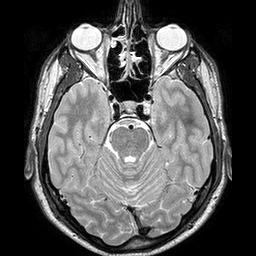
\includegraphics[width=.5\linewidth]{cerveau.jpg}}
 
 \subfloat[Gaussian pyramid le\-vel 1.]{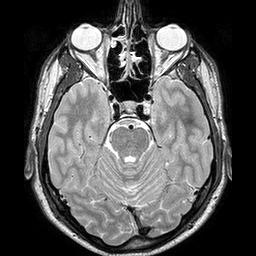
\includegraphics[width=.3\linewidth]{gaussian0.python.png}}\hfill
 \subfloat[Level 2.]{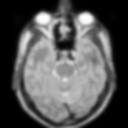
\includegraphics[width=.3\linewidth]{gaussian1.python.png}}\hfill
 \subfloat[Level 3.]{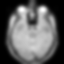
\includegraphics[width=.3\linewidth]{gaussian2.python.png}}

 \subfloat[Laplacian pyramid le\-vel 1.]{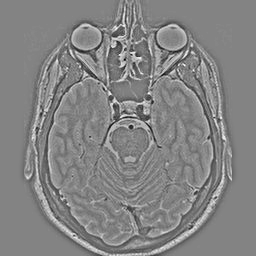
\includegraphics[width=.3\linewidth]{laplacian0.python.png}}\hfill
 \subfloat[Level 2.]{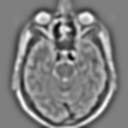
\includegraphics[width=.3\linewidth]{laplacian1.python.png}}\hfill
 \subfloat[Level 3.]{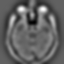
\includegraphics[width=.3\linewidth]{laplacian2.python.png}}%
 \label{fig:multiscale:python:glpyramid}%
\end{figure}

\subsubsection{Reconstruction}
The reconstruction is straighforward and exact because of the construction of the residue. The details can be filtered (removed for example), thus giving the following result Fig. \ref{fig:multiscale:python:nodetails}.

\begin{python}
def LaplacianPyramidReconstruction(pyr, interp='bilinear'):
    """
    Reconstruction of the Laplacian pyramid, starting from the last image
    pyr: pyramid of images (list of arrays)
    interp: interpolation mode, for upsizing the image
    returns: Image, reconstructed image
    """
    
    Image = pyr[-1];
    for i in range(len(pyr)-2, -1, -1):
        Image = pyr[i] + misc.imresize(Image, pyr[i].shape, interp=interp, mode='F');
        
    return Image;
\end{python}

\begin{figure}[htbp]
\centering\caption{Reconstruction of the Laplacian pyramid.}%
 \subfloat[Reconstruction of the pyramid without any detail.]{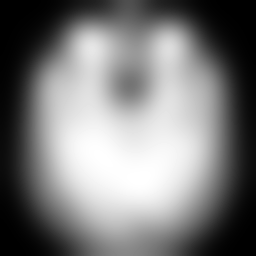
\includegraphics[width=.4\linewidth]{lPyrnodetails.python.png}}\hfill
 \subfloat[Reconstruction of the pyramid with all the details.]{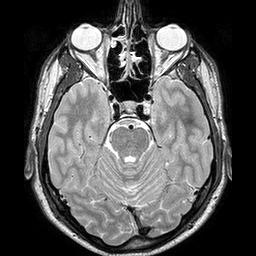
\includegraphics[width=.4\linewidth]{lPyrRec.python.png}}%
 \label{fig:multiscale:python:nodetails}
\end{figure}


\subsection{Scale-space decomposition and multiscale filtering}
The pyramid of erosions and dilations is illustrated in Fig.\ref{fig:multiscale:python:erodil}.
\begin{python}
def morphoMultiscale(I, levels):
    """
    Morphological multiscale decomposition
    I: original image, float32
    levels: number of levels, int
    
    returns: pyrD, pyrE: pyramid of Dilations/Erosions, respectively
    """
    pyrD=[];
    pyrE=[];
    for r in np.arange(1,levels):
        se = morphology.disk(r);
        pyrD.append( morphology.dilation(I, selem=se));
        pyrE.append( morphology.erosion(I, selem=se));
    return pyrD, pyrE;
\end{python}


\begin{figure}[htbp]
\centering\caption{Morphological multiscale decomposition by dilation and erosion.}%
 \subfloat[Dilation scale 1.]{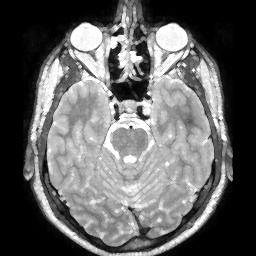
\includegraphics[width=.3\linewidth]{dilation0.python.png}}\hfill
 \subfloat[Dilation scale 2.]{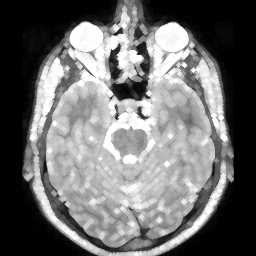
\includegraphics[width=.3\linewidth]{dilation1.python.png}}\hfill
 \subfloat[Dilation scale 3.]{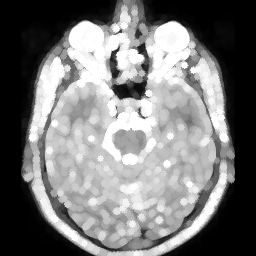
\includegraphics[width=.3\linewidth]{dilation2.python.png}} 
 
 \subfloat[Erosion scale 1.]{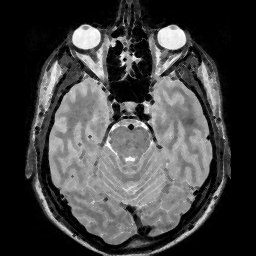
\includegraphics[width=.3\linewidth]{erosion0.python.png}}\hfill
 \subfloat[Erosion scale 2.]{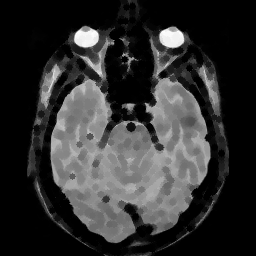
\includegraphics[width=.3\linewidth]{erosion2.python.png}}\hfill
 \subfloat[Erosion scale 3.]{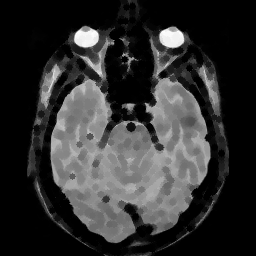
\includegraphics[width=.3\linewidth]{erosion2.python.png}}%
 \label{fig:multiscale:python:erodil}%
\end{figure}

\subsection{Kramer and Bruckner multiscale decomposition}
The results are illustrated in Fig.\ref{fig:multiscale:python:KB}.

\begin{figure}[htbp]
\centering\caption{Kramer and Bruckner multiscale decomposition, with $r=5$.}%
 \subfloat[$MK_B^1$.]{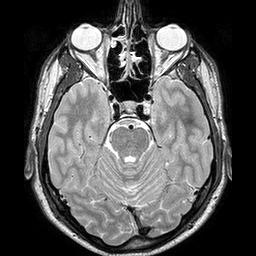
\includegraphics[width=.3\linewidth]{mkb0.python.png}}\hfill
 \subfloat[$MK_B^2$.]{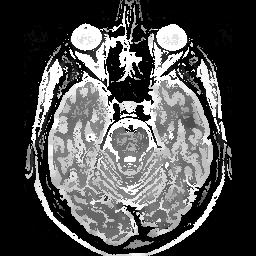
\includegraphics[width=.3\linewidth]{mkb1.python.png}}\hfill
 \subfloat[$MK_B^3$.]{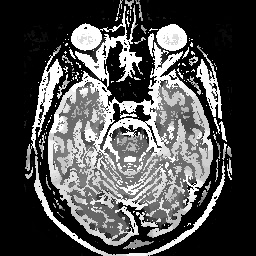
\includegraphics[width=.3\linewidth]{mkb2.python.png}}%
 \label{fig:multiscale:python:KB}%
\end{figure}

\begin{python}
def kb(I, r):
    """
    Elementary Kramer/Bruckner filter. Also called toggle filter.
    I: image
    r: radius of structuring element (disk), for max/min evaluation
    """
    se = morphology.disk(r);
    D=morphology.dilation(I, selem=se);
    E=morphology.erosion(I, selem=se);
    difbool = D-I < I-E; 
    k = D*difbool + E * (~difbool);
    return k;
\end{python}

\begin{python}
def KBmultiscale(I, levels, r=1):
    """
    Kramer and Bruckner multiscale decomposition
    
    I: original image, float32
    pyrD: pyramid of Dilations
    pyrE: pyramid of Erosions
    
    returns: MKB: Kramer/Bruckner filters
    """
    MKB = [];
    MKB.append(I);
    for i in range(levels):
        MKB.append(kb(MKB[i-1], r));
    return MKB
\end{python}

